% =====================================================================
%  A modularity-matrix equivalent of the Fiedler value
%  Reply to the meeting of Monday 31 August 2026.
%  Self-contained: no .bib, no \includegraphics, no external data.
%  Compiles on Overleaf as-is, and locally with:
%      tectonic -X compile reports/2026-09-08_modularity_equivalence.tex
%  Every number is printed by modularity_indicator/report_numbers.py
% =====================================================================
\documentclass[11pt,a4paper]{article}

\usepackage[T1]{fontenc}
\usepackage[utf8]{inputenc}
\usepackage{lmodern}
\usepackage[margin=2.3cm]{geometry}
\usepackage{amsmath,amssymb}
\usepackage{booktabs}
\usepackage{array}
\usepackage{enumitem}
\usepackage{xcolor}
\usepackage{microtype}
\usepackage{caption}
\usepackage{tikz}
\usetikzlibrary{positioning,arrows.meta,calc,fit,backgrounds}
\usepackage{pgfplots}
\pgfplotsset{compat=1.18}

\definecolor{BlueLink}{HTML}{1F4E79}
\definecolor{BadRed}{HTML}{B3261E}
\definecolor{ModC}{HTML}{1F4E79}   % modularity family
\definecolor{LapC}{HTML}{2F6F4E}   % Laplacian family
\definecolor{CorrC}{HTML}{7A6A55}  % scale / degree family
\definecolor{ScalC}{HTML}{B3261E}
\definecolor{Panel}{HTML}{EDEFF2}
\definecolor{Panel2}{HTML}{F7F5F0}
\definecolor{Rule}{HTML}{9AA3AD}

\usepackage[colorlinks=true,linkcolor=BlueLink,urlcolor=BlueLink]{hyperref}
\emergencystretch=3em

\newcommand{\Lap}{\mathbf{L}}
\newcommand{\Amat}{\mathbf{A}}
\newcommand{\Bmat}{\mathbf{B}}
\newcommand{\Dmat}{\mathbf{D}}
\newcommand{\dvec}{\mathbf{d}}
\newcommand{\Lsym}{\Lap_{\mathrm{sym}}}
\newcommand{\Bn}{\Bmat_{n}}

\captionsetup{font=small,labelfont=bf,width=.94\textwidth}
\setlist[itemize]{topsep=3pt,itemsep=2pt,parsep=0pt,leftmargin=1.3em}
\setlist[enumerate]{topsep=3pt,itemsep=2pt,parsep=0pt,leftmargin=1.8em}
\setlength{\parskip}{3pt}
\pagestyle{plain}

\newsavebox{\asidebox}
\newenvironment{aside}[1]
 {\par\vspace{2.5mm}\begin{lrbox}{\asidebox}%
  \begin{minipage}{\dimexpr\textwidth-16pt\relax}\small\textbf{#1}\par\vspace{1mm}}
 {\end{minipage}\end{lrbox}%
  \noindent\setlength{\fboxsep}{7pt}\setlength{\fboxrule}{.4pt}%
  \fcolorbox{Rule}{Panel2}{\usebox{\asidebox}}\par\vspace{2.5mm}}

\begin{document}

\begin{center}
{\Large\textbf{A modularity-matrix equivalent of the Fiedler value}}\\[2mm]
{\normalsize Jash Dalal \quad$\cdot$\quad 8 September 2026}\\[1mm]
{\small Reply to the meeting of Monday 31 August. Tested exclusively on Paper 1's
FAAMUNG data, as agreed.\\ Code in \texttt{modularity\_indicator/}; every number
below is printed by \texttt{modularity\_indicator/report\_numbers.py}.}
\end{center}
\vspace{2mm}
\hrule
\vspace{4mm}

% =====================================================================
\section{The question, and the answer in one page}
% =====================================================================

Paper 1 (Cardoso \& Palomar 2020) learns a graph Laplacian $\Lap_t$ directly from
returns on rolling 30-day windows and reads one number off it: the Fiedler value
$\lambda_2(\Lap_t)$, which measures how tightly the network holds together and is
used as a market-stress indicator. The task set on 31 August was to find a
quantity derived from the \textbf{modularity matrix}
$\Bmat = \Amat - \dvec\dvec^{\!\top}\!/2m$ that carries the same information, tested
on Paper 1's own data, as a first step toward a theory-backed account of what the
spectra of these matrices encode.

\textbf{Method.} Paper 1 discards the learned graphs after extracting $\lambda_2$,
so Algorithm 2 was re-run with its exact constants to recover all
$\mathbf{243}$ Laplacians, and the weighted adjacency recovered as
$\Amat_t = -\operatorname{offdiag}(\Lap_t)$. From each, 22 modularity-derived
quantities were computed alongside 6 Laplacian references, and each candidate was
scored on the four things Paper 1 actually uses $\lambda_2$ for: agreement with
$\lambda_2$, agreement of the trading gate, behaviour into the COVID crash, and
the S1/S2 backtest. Two gates passed first: the recomputed $\lambda_2$ matches
Paper 1's cached series to $1.2\times10^{-10}$, and the backtest reproduces its
published $S1 = +0.0779$ against $S2 = -0.0111$.

\textbf{Result.} The question as posed has a clean negative answer, in two parts.

\begin{aside}{The two-part answer}
\textbf{(i) Normalise, and the question dissolves.} After degree normalisation the
modularity matrix and the Laplacian are \emph{the same operator}: they share an
eigenbasis exactly, and their eigenvalues are in one-to-one correspondence
$\mu = 1-\lambda$. Verified across the full spectrum on all 243 windows to
$1.8\times10^{-15}$. Any indicator built from normalised $\Bmat$ is therefore a
Laplacian indicator in different notation. This is a proof, not a measurement.

\smallskip
\textbf{(ii) Do not normalise, and the natural shortcut is unsound.} The candidate
that topped our table, $\bar{d}-\mu_1(\Bmat)$, rests on an identity that holds
only when \emph{every} degree is equal. Substituting the \emph{mean} degree is not
a weakened hypothesis; it is no hypothesis. Its error is $89\%$ as large as
$\lambda_2$'s own standard deviation. This is the point raised at the meeting, and
it is confirmed quantitatively in \S4.
\end{aside}

Three further findings came out of chasing that answer down, and they are worth
more than the original question was.

\begin{enumerate}[label=\textbf{\arabic*.}]
\item \textbf{Correlation, the metric we screened candidates with, is the wrong
test for novelty.} It promoted the spurious candidate in (ii) to the top of the
table, and it independently fails to flag a quantity that is provably pure
tautology (\S5).
\item \textbf{Under Paper 1's own experimental conditions, $\lambda_2$ sits inside
the noise band.} It beats a random \emph{day}, but not a random 24-day
\emph{stretch}: COVID lands at the 76th percentile of the sliding-event null,
$p=0.243$ (\S6). Matching $\lambda_2$ was therefore never a well-defined target.
\item \textbf{$\lambda_2$ splits into a structure part and a degree part, and the
degree part is where $\Bmat$ and $\Lap$ actually differ.} Degree information
detects nothing on its own (AUC $0.537$, a coin flip) yet \emph{improves} detection
when combined with structure, and it is exactly what normalisation destroys
(\S7). This localises where anything new can live, and reframes the project.
\end{enumerate}

The natural first move is the one in (i): normalise both matrices and compare
like with like. That is where the argument starts.

% =====================================================================
\section{Degree normalisation, and why it collapses the question}
% =====================================================================

\subsection*{What degree normalisation is}

The \textbf{degree} $d_i = \sum_j A_{ij}$ is the total strength of stock $i$'s
connections. The raw matrices $\Amat$ and $\Lap$ mix two different things: how
\emph{much} a node is connected (its size), and how that connection is
\emph{distributed} across its neighbours (its shape). A heavily connected stock
dominates every spectral quantity simply because its numbers are larger.

Degree normalisation divides that out. Each entry becomes
\[
A_{ij} \;\longmapsto\; \frac{A_{ij}}{\sqrt{d_i d_j}},
\]
so every edge is measured relative to how connected its two endpoints already
are. A weight of $0.5$ between two hubs is small; the same $0.5$ between two
peripheral stocks is large.

\begin{aside}{The analogy that makes this exact}
Normalisation is to $\Lap$ what \textbf{correlation} is to \textbf{covariance}.
Covariance mixes each series' volatility with their co-movement; dividing by
$\sigma_i\sigma_j$ strips out the volatilities so only co-movement remains. Here,
dividing by $\sqrt{d_i d_j}$ strips out the degrees so only structure remains.
Same operation, same purpose.
\end{aside}

Writing $\Dmat = \operatorname{diag}(d_1,\dots,d_n)$, the two normalised objects are
\[
\Lsym = \Dmat^{-1/2}\Lap\,\Dmat^{-1/2} = \mathbf{I} - \mathbf{N},
\qquad
\Bn = \Dmat^{-1/2}\Bmat\,\Dmat^{-1/2},
\qquad
\mathbf{N} = \Dmat^{-1/2}\Amat\,\Dmat^{-1/2}.
\]
The tell that the units are gone: doubling every edge weight doubles $\Lap$ but
leaves $\Lsym$ untouched, and $\Lsym$'s eigenvalues always lie in $[0,2]$.

\subsection*{The two normalised matrices are the same operator}

Normalising the null term gives entries $\sqrt{d_i d_j}/2m$, which is exactly
$\mathbf{u}\mathbf{u}^{\!\top}$ for the unit vector
$\mathbf{u} = \Dmat^{1/2}\mathbf{1}/\sqrt{2m}$, so
\[
\boxed{\;\Bn \;=\; \mathbf{N} - \mathbf{u}\mathbf{u}^{\!\top}\;}
\qquad\text{and}\qquad
\mathbf{N}\mathbf{u} = \mathbf{u},
\]
since $(\mathbf{N}\mathbf{u})_i = \sum_j \tfrac{A_{ij}}{\sqrt{d_id_j}}\sqrt{\tfrac{d_j}{2m}}
= \tfrac{d_i}{\sqrt{2m\,d_i}} = u_i$. So $\mathbf{u}$ is $\mathbf{N}$'s Perron
eigenvector, and $\Bn$ does exactly one thing to $\mathbf{N}$: it deflates that one
mode to zero and leaves every other eigenpair untouched. Hence
\[
\operatorname{spec}(\Bn) \;=\; \{0\}\cup\{\,1-\lambda_i(\Lsym)\,\}_{i\ge2},
\qquad\text{with the \emph{same} eigenvectors.}
\]
Equivalently $\Bn = \mathbf{I} - \Lsym - \mathbf{u}\mathbf{u}^{\!\top}$, where
$\mathbf{u}$ is itself $\Lsym$'s null vector: $\Bn$ is a closed-form function of
$\Lsym$ alone. Measured on all 243 windows:

\begin{center}\small
\renewcommand{\arraystretch}{1.15}
\begin{tabular}{@{}lr@{}}
\toprule
\textbf{Check (243 windows)} & \textbf{Result} \\
\midrule
$\max\big|\operatorname{spec}(\Bn) - (\{0\}\cup\{1-\lambda_i(\Lsym)\})\big|$ &
$1.8\times10^{-15}$ \\
$\max\big|\mu_1(\Bn) - (1-\lambda_2(\Lsym))\big|$ & $1.3\times10^{-15}$ \\
eigenvector agreement, $\Bn$ vs $\Lsym$ (mean best overlap) &
$\mathbf{1.000000}$ \quad(min $1.000000$) \\[2pt]
\textit{for contrast:} eigenvector agreement, $\Bmat$ vs $\Lap$ &
$0.871$ \quad(min $0.786$) \\
\textit{for contrast:} $|\langle$Fiedler vector of $\Lap$, top eigenvector of
$\Bmat\rangle|$ & $0.728$ \quad(range $[0.039,\,0.974]$) \\
\bottomrule
\end{tabular}
\end{center}

Two things deserve emphasis. First, the pairing \textbf{reverses the order}:
$\lambda_2$ is near the \emph{bottom} of the Laplacian spectrum, and its twin
$\mu_1$ is at the \emph{top} of the modularity spectrum. That is why the
correspondence is not obvious by inspection, but it also means ``read the top
of $\Bmat$ instead of the bottom of $\Lap$'' is the same idea backwards, not a new
one. Second, the identity needs the graph \textbf{connected}, so that $\Lsym$ has a
one-dimensional null space and $\mathbf{u}$ is recoverable. Paper 1 enforces this
with $k=1$, so it holds on all 243 windows here; it would fail on a fragmented
graph, which is precisely the regime that broke the Paper 3 replication.

\begin{figure}[h]\centering
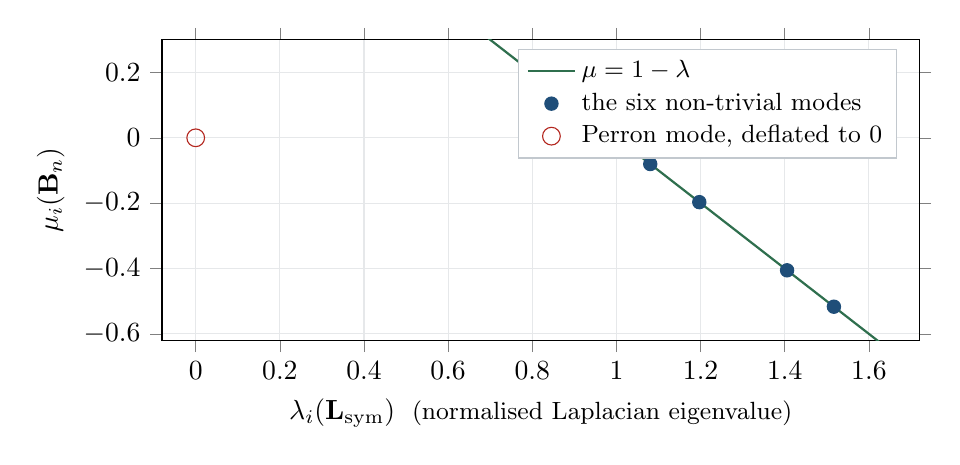
\begin{tikzpicture}
\begin{axis}[width=11.2cm,height=5.4cm,
  xlabel={$\lambda_i(\Lsym)$ \;\small(normalised Laplacian eigenvalue)},
  ylabel={$\mu_i(\Bn)$},
  xmin=-0.08,xmax=1.72,ymin=-0.62,ymax=0.30,
  grid=both,grid style={Rule!25},tick align=outside,
  legend cell align=left,legend pos=north east,legend style={draw=Rule!60,font=\small}]
\addplot[LapC,thick,domain=-0.05:1.7,samples=2]{1-x};
\addlegendentry{$\mu = 1-\lambda$}
\addplot[only marks,mark=*,mark size=2.4pt,ModC]
  coordinates {(0.8363,0.1637) (0.9642,0.0358) (1.0803,-0.0803)
               (1.1969,-0.1969) (1.4055,-0.4055) (1.5168,-0.5168)};
\addlegendentry{the six non-trivial modes}
\addplot[only marks,mark=o,mark size=3.2pt,BadRed] coordinates {(0.0000,0.0000)};
\addlegendentry{Perron mode, deflated to $0$}
\end{axis}
\end{tikzpicture}
\caption{The spectra of $\Bn$ and $\Lsym$ for one window (2020-03-16, Paper 1's
own COVID-crash snapshot). Every eigenvalue lies on the line $\mu = 1-\lambda$
exactly; the trivial mode is sent to $0$ rather than to $1$, which loses nothing
because $\lambda_1(\Lsym)=0$ always. The picture is identical on all 243 windows.}
\end{figure}

\textbf{Consequence.} No indicator derived from normalised $\Bmat$ can be new.
This closes a large part of the search permanently: not ``we tried and failed''
but ``this cannot work''. So the search must use the \emph{unnormalised} $\Bmat$.
Which raises the immediate question: how much of the menu we actually built was
normalised?

% =====================================================================
\section{The candidate menu, and how much of it was already decided}
% =====================================================================

Of the 28 quantities scored, 22 are modularity-derived. Splitting them by
provenance:

\begin{center}\small
\renewcommand{\arraystretch}{1.2}\setlength{\tabcolsep}{5pt}
\begin{tabular}{@{}>{\raggedright\arraybackslash}p{2.9cm}
                  >{\raggedright\arraybackslash}p{10.3cm}
                  >{\raggedright\arraybackslash}p{2.5cm}@{}}
\toprule
\textbf{Built from} & \textbf{Candidates} & \textbf{Status} \\
\midrule
\textcolor{ModC}{\textbf{normalised $\Bn$}} \newline (3) &
\texttt{mu1\_norm}, \texttt{muN\_norm}, \texttt{one\_minus\_mu1n} &
\textbf{tautological} by \S2 \\
\textcolor{ModC}{\textbf{plain $\Bmat$}} \newline (19) &
\texttt{mu1}, \texttt{mu2}, \texttt{muN}, \texttt{gap12}, \texttt{spread},
\texttt{mu\_ratio}, \texttt{absmax}, \texttt{n\_pos}, \texttt{trace\_pos},
\texttt{trace\_neg}, \texttt{energy}, \texttt{frob2}, \texttt{spec\_entropy},
\texttt{q\_bound}, \texttt{ipr1}, \texttt{iprN}, \texttt{v1\_deg\_align},
\texttt{dbar\_minus\_mu1}, \texttt{dual\_resid} & not settled by \S2 \\
\textcolor{LapC}{\textbf{Laplacian ref.}} \newline (6) &
\texttt{lam2}, \texttt{lam\_max}, \texttt{lam2\_sym}, \texttt{dbar},
\texttt{two\_m}, \texttt{deg\_cv} & baselines \\
\bottomrule
\end{tabular}
\end{center}

The three normalised candidates are not merely correlated with Laplacian
quantities; they are \emph{affine images} of them, so their correlation is
exactly $\pm1$:
\[
\operatorname{corr}\big(\mu_1(\Bn),\,\lambda_2(\Lsym)\big) = -1.0000000000,
\qquad
\operatorname{corr}\big(\mu_N(\Bn),\,\lambda_{\max}(\Lsym)\big) = -1.0000000000,
\]
and \texttt{one\_minus\_mu1n} equals $\lambda_2(\Lsym)$ to \emph{exactly} zero
error. They were included as consistency checks and they behaved as such.

There is a second, less expected collapse \emph{inside} the plain-$\Bmat$ block.
Several ``different'' candidates are one quantity relabelled:

\begin{center}\small
\renewcommand{\arraystretch}{1.1}
\begin{tabular}{@{}lrlr@{}}
\toprule
\multicolumn{4}{@{}l}{\textbf{Correlation with $\mu_1(\Bmat)$, 243 windows}}\\
\midrule
\texttt{spread} ($\mu_1-\mu_N$) & $+0.966$ & \texttt{energy} & $+0.891$ \\
\texttt{trace\_pos} ($\sum_{\mu>0}\mu$) & $+0.951$ & \texttt{mu\_ratio} & $-0.881$ \\
\texttt{gap12} ($\mu_1-\mu_2$) & $+0.935$ & \texttt{q\_bound} & $+0.793$ \\
\texttt{frob2} ($\operatorname{tr}\Bmat^2$) & $+0.898$ &
\textbf{\texttt{muN}} & $\mathbf{-0.668}$ \\
\bottomrule
\end{tabular}
\end{center}

So what looked like a table of five leading findings was largely $\mu_1(\Bmat)$
wearing different labels. (\texttt{absmax} is worse than a relabelling: since
$|\mu_N| > \mu_1$ on $243/243$ windows, it \emph{is} $|\mu_N|$.) The one plain-$\Bmat$
candidate that stands genuinely apart from the $\mu_1$ family is $\mu_N(\Bmat)$,
at $-0.668$; we return to it in \S8.

One plain-$\Bmat$ candidate topped the whole table on agreement with $\lambda_2$:
$\bar{d}-\mu_1(\Bmat)$, at $91\%$ agreement of daily invest/cash calls. That is
the one to examine next.

% =====================================================================
\section{The theorem that was assumed, and why it does not hold}
% =====================================================================

The motivation for $\bar{d}-\mu_1(\Bmat)$ is a genuine identity. On a
\textbf{$d$-regular} graph, one in which every node has the \emph{same} degree $d$, we have
$2m = nd$, so $\dvec\dvec^{\!\top}\!/2m = (d/n)\mathbf{1}\mathbf{1}^{\!\top}$ and
\[
\Bmat = d\mathbf{I} - \Lap - \tfrac{d}{n}\mathbf{1}\mathbf{1}^{\!\top}
\quad\Longrightarrow\quad
\mu_1(\Bmat) = d - \lambda_2(\Lap).
\]
The whole argument rests on $\Dmat = d\mathbf{I}$: a scalar multiple of the
identity commutes with everything and shifts every eigenvalue equally. For an
irregular graph the term is $\Dmat$, a diagonal matrix of \emph{different}
degrees, and there is no scalar to pull out. \textbf{Replacing $d$ by the mean
degree $\bar{d}$ is not a weakened hypothesis; it is no hypothesis at all}, and
the resulting discrepancy is whatever it happens to be. This is the objection
raised at the 31 August meeting, and it is why the $\lambda_2(\Lap)+\mu_1(\Bmat)=d$
spine proposed in the 12 August log (direction D2) was not pursued. Measuring it:

\begin{center}\small
\renewcommand{\arraystretch}{1.18}
\begin{tabular}{@{}>{\raggedright\arraybackslash}p{5.0cm}r
                  >{\raggedright\arraybackslash}p{7.3cm}@{}}
\toprule
\textbf{Diagnostic} & \textbf{Value} & \textbf{Reading} \\
\midrule
degree CV of these graphs & $0.305$ &
nowhere near regular ($0$ would be); range $[0.240,0.369]$, $\bar{d}=2.13$ \\
$\max|\operatorname{spec}(\Bmat)-(\{0\}\cup\{\bar d-\lambda_i(\Lap)\})|$ &
$\mathbf{1.25}$ & $5.3\times$ $\lambda_2$'s own sd of $0.235$. Not an identity \\
residual $r=(\bar d-\mu_1)-\lambda_2$, sd & $0.208$ &
$\mathbf{89\%}$ of $\lambda_2$'s sd; the error is as large as the signal \\
residual, mean and range & $0.492$, $[0.145,0.971]$ &
varies six-fold, so not a constant offset that could be subtracted \\
$\operatorname{corr}(r,\lambda_2)$ & $+0.395$ &
the error moves \emph{with} the signal, inflating the apparent fit \\
$\operatorname{corr}(r,\text{degree CV})$ & $+0.020$ &
not a simple ``more irregular $\Rightarrow$ bigger error'' effect: no correction available \\
residual in-crash vs out & $0.308$ vs $0.512$ &
the error is \emph{event-dependent}; part of the crash tracking is the error term \\
\bottomrule
\end{tabular}
\end{center}

Decomposing the variance of the proxy itself, $\bar d - \mu_1 = \lambda_2 + r$:
\textbf{only $40\%$ comes from $\lambda_2$}, $32\%$ from the residual, $28\%$ from
their covariance. Less than half of the movement in the proposed indicator is the
quantity it was standing in for.

\begin{figure}[h]\centering
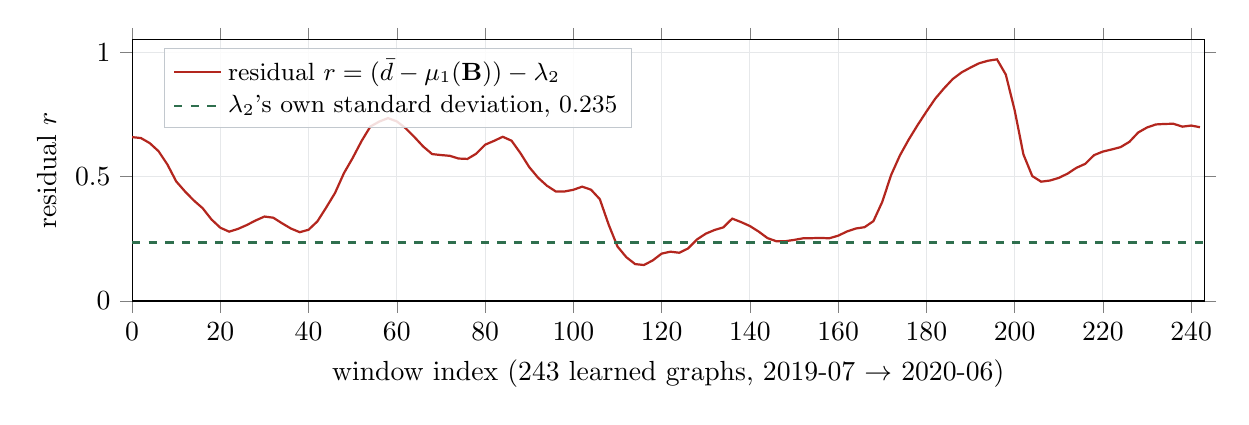
\begin{tikzpicture}
\begin{axis}[width=15.2cm,height=4.9cm,
  xlabel={window index (243 learned graphs, 2019-07 $\to$ 2020-06)},
  ylabel={residual $r$},
  xmin=0,xmax=243,ymin=0,ymax=1.05,
  grid=both,grid style={Rule!25},tick align=outside,
  legend cell align=left,legend pos=north west,
  legend style={draw=Rule!60,font=\small,fill=white,fill opacity=0.85,text opacity=1}]
\addplot[BadRed,thick] coordinates {
(0,0.6587) (2,0.6551) (4,0.6347) (6,0.6022) (8,0.5490) (10,0.4809) (12,0.4403)
(14,0.4041) (16,0.3730) (18,0.3278) (20,0.2947) (22,0.2789) (24,0.2899) (26,0.3055)
(28,0.3238) (30,0.3396) (32,0.3349) (34,0.3124) (36,0.2914) (38,0.2767) (40,0.2866)
(42,0.3202) (44,0.3760) (46,0.4345) (48,0.5135) (50,0.5751) (52,0.6428) (54,0.7013)
(56,0.7211) (58,0.7351) (60,0.7219) (62,0.6943) (64,0.6587) (66,0.6206) (68,0.5906)
(70,0.5867) (72,0.5836) (74,0.5727) (76,0.5711) (78,0.5923) (80,0.6282) (82,0.6435)
(84,0.6601) (86,0.6443) (88,0.5946) (90,0.5383) (92,0.4958) (94,0.4636) (96,0.4406)
(98,0.4403) (100,0.4471) (102,0.4597) (104,0.4475) (106,0.4094) (108,0.3072)
(110,0.2192) (112,0.1763) (114,0.1485) (116,0.1448) (118,0.1634) (120,0.1906)
(122,0.1984) (124,0.1941) (126,0.2113) (128,0.2473) (130,0.2707) (132,0.2856)
(134,0.2961) (136,0.3313) (138,0.3174) (140,0.3015) (142,0.2791) (144,0.2529)
(146,0.2404) (148,0.2405) (150,0.2456) (152,0.2520) (154,0.2527) (156,0.2535)
(158,0.2523) (160,0.2626) (162,0.2795) (164,0.2915) (166,0.2969) (168,0.3212)
(170,0.3985) (172,0.5061) (174,0.5853) (176,0.6490) (178,0.7068) (180,0.7611)
(182,0.8131) (184,0.8548) (186,0.8926) (188,0.9191) (190,0.9383) (192,0.9558)
(194,0.9658) (196,0.9712) (198,0.9101) (200,0.7669) (202,0.5888) (204,0.5022)
(206,0.4797) (208,0.4843) (210,0.4949) (212,0.5121) (214,0.5354) (216,0.5514)
(218,0.5864) (220,0.6007) (222,0.6092) (224,0.6185) (226,0.6397) (228,0.6773)
(230,0.6975) (232,0.7097) (234,0.7117) (236,0.7124) (238,0.7008) (240,0.7052)
(242,0.6986)};
\addlegendentry{residual $r = (\bar d-\mu_1(\Bmat))-\lambda_2$}
\addplot[LapC,dashed,thick,domain=0:243,samples=2]{0.2351};
\addlegendentry{$\lambda_2$'s own standard deviation, $0.235$}
\end{axis}
\end{tikzpicture}
\caption{If $\bar d-\mu_1(\Bmat)$ were a usable proxy for $\lambda_2$, this
residual would be flat and small. It is neither: it swings from $0.15$ to $0.97$,
with a standard deviation $89\%$ as large as $\lambda_2$'s own. It is also
systematically \emph{lower} through the COVID window (indices $150$--$173$),
averaging $0.308$ there against $0.512$ outside, so part of what looked like
crash tracking was the error term moving, not the identity holding.}
\end{figure}

\textbf{The $\bar d$ term was never doing any work.} Controlling for graph scale,
$\mu_1(\Bmat)$ on its own tracks $\lambda_2$ exactly as well as the proxy does:

\begin{center}\small
\begin{tabular}{@{}lrr@{}}
\toprule
& \textbf{raw} & \textbf{partial, given $\bar d$} \\
\midrule
$\operatorname{corr}(\lambda_2,\ \mu_1(\Bmat))$ & $-0.574$ & $\mathbf{-0.851}$ \\
$\operatorname{corr}(\lambda_2,\ \bar d-\mu_1(\Bmat))$ & $+0.856$ & $\mathbf{+0.851}$ \\
\bottomrule
\end{tabular}
\end{center}

Identical. The subtraction only inflated the headline correlation by importing a
scale nuisance; it contributed nothing conditional. The honest, defensible
statement that survives is a regression fact with no theorem attached: \emph{at
fixed graph scale, $\mu_1(\Bmat)$ tracks $\lambda_2$ at $-0.85$.}

\begin{aside}{On the two correlation figures in the record}
$\operatorname{corr}(\lambda_2,\ \bar d-\mu_1)$ is $0.856$ over all 243 learned
graphs and $0.882$ over the 201-day evaluation window. Both are correct; the
earlier note quoted the second. All \emph{detection} numbers in this report are on
the 201-day window (that is where the backtest lives); all \emph{structural}
numbers are on all 243.
\end{aside}

This leaves an uncomfortable question. A quantity with no valid derivation scored
the highest agreement with $\lambda_2$ of anything we tested. Why did our
screening let it through?

% =====================================================================
\section{Why correlation is the wrong test for novelty}
% =====================================================================

Correlation with $\lambda_2$ was adopted early as the working metric for comparing
$\Bmat$-derived quantities against $\Lap$-derived ones, and it is the first column
of every table we produced. It is a reasonable measure of \emph{agreement}. It is
not a measure of \emph{novelty}, and novelty is what the question was about.

\begin{aside}{What ``novelty'' means here: the definition this report commits to}
A modularity-derived quantity is \textbf{new} if and only if it \textbf{cannot be
reconstructed from $\operatorname{spec}(\Lap)$}. If it can, then whatever it
measures was already available on the Laplacian side, and calling it a modularity
indicator is a relabelling.

\smallskip
\emph{Necessary caveat.} $\Lap$ determines $\Amat$ determines $\Bmat$, so at the
level of \emph{matrices} everything here is recoverable from everything else and
the question is empty. The claim is strictly about \textbf{spectra}, which is where
indicators actually live: $\operatorname{spec}(\Bn)$ is a bijection of
$\operatorname{spec}(\Lsym)$ (\S2), whereas $\operatorname{spec}(\Bmat)$ is not a
bijection of $\operatorname{spec}(\Lap)$, and they do not even share an eigenbasis
(overlap $0.871$, and on some windows the two leading modes are nearly orthogonal
at $0.039$).
\end{aside}

Correlation fails against that definition in both directions.

\medskip
\noindent\textbf{Direction 1: it accepts things that are pure tautology.}
Correlation only detects an \emph{affine} relationship. When the map from a
Laplacian quantity to a modularity quantity is affine, correlation catches it
perfectly; when the map is non-linear, correlation goes quiet even though the
quantity contains literally no new information.

\begin{center}\small
\renewcommand{\arraystretch}{1.2}
\begin{tabular}{@{}lrr@{}}
\toprule
\textbf{Quantity of $\Bn$} & \textbf{corr.\ with $\lambda_2$} &
\textbf{error when rebuilt from $\operatorname{spec}(\Lsym)$ alone} \\
\midrule
$\mu_1(\Bn)$ \quad\small(affine: $1-\lambda_2$) & $-1.0000000000$ & n/a (exact by construction) \\
nuclear norm $\|\Bn\|_*$ & $-0.834$ & $2.7\times10^{-15}$ \\
\textbf{spectral entropy of $\Bn$} & $\mathbf{-0.264}$ & $\mathbf{8.0\times10^{-15}}$ \\
\bottomrule
\end{tabular}
\end{center}

The last row is the whole point. Spectral entropy of $\Bn$ correlates only
$-0.264$ with $\lambda_2$. On a correlation screen it looks like an independent
signal and would have been promoted as a discovery. It was rebuilt here from the
$\Lsym$ spectrum alone, with no access to $\Bmat$ at any stage, to
$8.0\times10^{-15}$. It carries exactly zero new information.

\medskip
\noindent\textbf{Direction 2: it promotes things that are spurious.} That is
\S4: the candidate with the single highest correlation in the study, $0.882$, had
no valid derivation, and $40\%$ of its variance was the target while $32\%$ was
error.

\medskip
\noindent\textbf{The practical consequence.} \emph{Low correlation with $\lambda_2$
is not evidence of new information, and high correlation is not evidence of a
sound relationship.} $\lambda_2$ is one scalar summary of a spectrum; a non-linear
re-reading of that same spectrum will decorrelate from it while adding nothing.
Novelty has to be argued from what a quantity is a \emph{function of}, not from how
it correlates, which is why the criterion in the box above is stated in terms of
reconstructibility.

Both directions of the test, though, measure candidates against $\lambda_2$. That
presumes $\lambda_2$ is a sound target. It is worth checking whether it is.

% =====================================================================
\section{$\lambda_2$ under Paper 1's own experimental conditions}
% =====================================================================

\subsection*{The setup, stated precisely}

\begin{center}\small
\renewcommand{\arraystretch}{1.15}
\begin{tabular}{@{}ll@{}}
\toprule
universe & 7 stocks (META, AAPL, AMZN, MSFT, UBER, NFLX, GOOGL) \\
sample & 272 trading days, 2019-06-04 $\to$ 2020-06-30 \\
graphs & 243 causal rolling windows, 30 days each; $k=1$, $\eta=0$,
$\beta=0$, $\delta=100$ \\
evaluation window & 201 signal days, 2019-07-16 $\to$ 2020-05-01 (exp4's window) \\
events & \textbf{one}: COVID, 2020-02-19 $\to$ 2020-03-23, giving \textbf{24 crash days} \\
rule & invest when $\lambda_2 < \tau = 1.0$; that gate invests $79/201$ days ($39.3\%$) \\
outcome & $S1$ (buy \& hold) $= +0.0779$; \quad $S2$ ($\lambda_2$ gate) $= -0.0111$ \\
\bottomrule
\end{tabular}
\end{center}

Seven stocks and a single event. That is the entire evidential base for the
indicator, and it bounds what any comparison against it can establish.

\subsection*{$\lambda_2$ sits inside the noise band}

\begin{enumerate}[label=\textbf{\alph*.}]
\item \textbf{The raw indicator scores below chance.} At raw levels, $\lambda_2$'s
COVID AUC is $\mathbf{0.472}$. FAAMUNG's autumn-2019 regime is already elevated, so
quiet days outrank crash days. Only after applying a strictly-prior 60-day
trailing $z$-score does it reach $0.759$. The published indicator, used as
published, does not separate the crash.

\item \textbf{It beats a random day, but not a random stretch.} These are different
nulls and they disagree:
\begin{center}\small
\begin{tabular}{@{}lll@{}}
\toprule
\textbf{Null} & \textbf{Result} & \textbf{Verdict} \\
\midrule
bootstrap over days & AUC $0.759$, 95\% CI $[0.634,\,0.875]$ &
excludes $0.5$: \textcolor{LapC}{\textbf{passes}} \\
sliding 24-day event window & COVID at the \textbf{76th percentile},
$p = \mathbf{0.243}$ & \textcolor{BadRed}{\textbf{fails}} \\
& \small null median $0.434$, 95th pct.\ $0.925$, max $0.963$ & \\
\bottomrule
\end{tabular}
\end{center}
$\lambda_2$ does rank crash days above calm days. What it cannot do is
distinguish COVID from an arbitrary volatile 24-day stretch of the same series,
which is what a crash \emph{detector} is supposed to do.

\item \textbf{The trading result is consistent with luck.} A uniform random gate at
the same invest rate beats buy-and-hold $\mathbf{39.2\%}$ of the time, so across 28
candidates roughly $11$ were expected to beat $S1$ by chance alone; $5$ did. A
circular-shift null preserving each signal's own autocorrelation clears nothing:
the best-performing candidate, $\operatorname{tr}(\Bmat^2)$ at $S2=+0.127$, has
$p = 0.305$, and the smallest $p$-value achieved by any candidate is $0.115$.

\item \textbf{No multiplicity correction exists anywhere in this study.} 28
quantities were scored against a single event. Nothing in this report, ours or
Paper 1's, should be read as a corrected significance claim.
\end{enumerate}

\begin{figure}[h]\centering
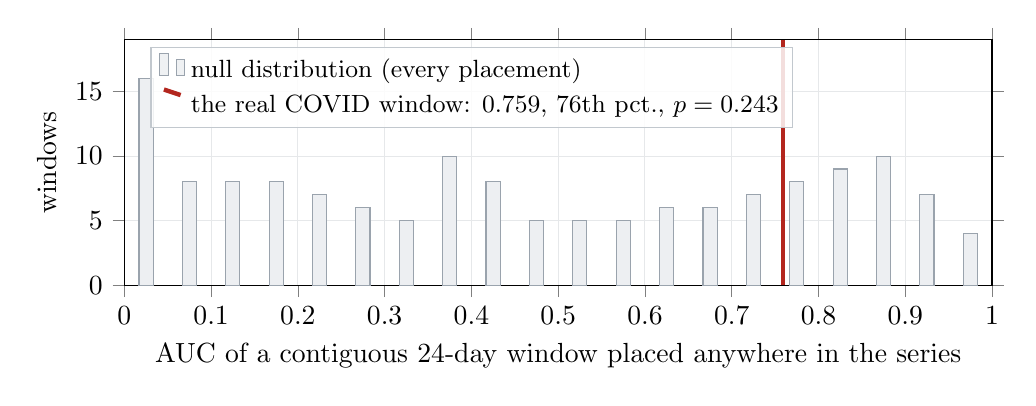
\begin{tikzpicture}
\begin{axis}[width=12.6cm,height=4.7cm,ybar,bar width=5.1pt,
  xlabel={AUC of a contiguous 24-day window placed anywhere in the series},
  ylabel={windows},
  xmin=0,xmax=1,ymin=0,ymax=19,
  grid=both,grid style={Rule!25},tick align=outside,
  legend cell align=left,legend pos=north west,
  legend style={draw=Rule!60,font=\small,fill=white,fill opacity=0.85,text opacity=1}]
\addplot[draw=Rule,fill=Panel] coordinates {
(0.025,16) (0.075,8) (0.125,8) (0.175,8) (0.225,7) (0.275,6) (0.325,5) (0.375,10)
(0.425,8) (0.475,5) (0.525,5) (0.575,5) (0.625,6) (0.675,6) (0.725,7) (0.775,8)
(0.825,9) (0.875,10) (0.925,7) (0.975,4)};
\addlegendentry{null distribution (every placement)}
\addplot[BadRed,ultra thick,sharp plot,update limits=false]
  coordinates {(0.759,0) (0.759,19)};
\addlegendentry{the real COVID window: $0.759$, 76th pct., $p=0.243$}
\end{axis}
\end{tikzpicture}
\caption{The sliding-event null for $\lambda_2$'s $z$-scored detector. If
$\lambda_2$ were specific to COVID, the red line would sit in the far right tail.
It sits inside the bulk: roughly a quarter of arbitrary 24-day windows score at
least as well.}
\end{figure}

\textbf{Consequence for the original question.} Matching $\lambda_2$ was never a
well-posed target, because $\lambda_2$'s own status on this data is not
established. The productive move is not to find something that agrees with it, but
to ask what it is \emph{made of}.

% =====================================================================
\section{Decomposing $\lambda_2$ into structure and degree}
% =====================================================================

\subsection*{How the split is defined}

The key observation is that Paper 1's indicator is read off the \textbf{unnormalised}
$\Lap$. By \S2, normalisation removes exactly two things: overall scale, and the
spread of degrees across nodes. So $\lambda_2(\Lap)$ is not a pure structure
measure. It is a blend of:

\begin{itemize}
\item a \textbf{structure} part, isolated by $\lambda_2(\Lsym)$, which is scale-free
by construction; and
\item a \textbf{scale/degree} part, carried by $\bar d$ (equivalently $2m$) and by
the degree spread \texttt{deg\_cv}.
\end{itemize}

Two ways to check that this split is real and not an artefact of the fit:

\begin{center}\small
\renewcommand{\arraystretch}{1.15}
\begin{tabular}{@{}lrr@{}}
\toprule
& \textbf{all 243 graphs} & \textbf{201-day window} \\
\midrule
$\operatorname{corr}(\lambda_2(\Lap),\ \lambda_2(\Lsym))$ \quad\small structure &
$+0.784$ & $+0.887$ \\
$\operatorname{corr}(\lambda_2(\Lap),\ \bar d)$ \quad\small scale &
$+0.489$ & $+0.743$ \\
$R^2$ of $\lambda_2(\Lap) \sim \lambda_2(\Lsym) + \bar d$ & $0.837$ & $0.848$ \\
\bottomrule
\end{tabular}
\end{center}

A regression alone would be weak evidence. The containment is exact, however:
\[
d_{\min}\cdot\lambda_2(\Lsym) \;\le\; \lambda_2(\Lap) \;\le\; d_{\max}\cdot\lambda_2(\Lsym)
\]
\textbf{holds on $243/243$ windows}, with $\lambda_2$ sitting $0.24$ of the way
across a band of mean width $1.351$ (sd of that position, $0.06$). So
``$\lambda_2 = $ structure $\times$ scale'' is a structural statement, not a fitted
one: the structure term sets the value up to a factor bounded by the degree range.

\subsection*{What each part detects}

Each component was put through the same detector (strictly-prior 60-day $z$-score,
direction fixed by correlation with $\lambda_2$, never by what scores best) and
scored on the same 24 COVID days:

\begin{center}\small
\renewcommand{\arraystretch}{1.2}
\begin{tabular}{@{}llrr@{}}
\toprule
\textbf{Quantity} & \textbf{What it is} & \textbf{AUC ($z$)} & \textbf{AUC (raw)} \\
\midrule
$\lambda_2(\Lap)$ & the full indicator, unnormalised & $\mathbf{0.759}$ & $0.472$ \\
$\lambda_2(\Lsym)$ & \textcolor{LapC}{structure only} & $0.700$ & $0.594$ \\
$\bar d$ & \textcolor{CorrC}{scale only} & $0.537$ & $0.156$ \\
$2m$ & \textcolor{CorrC}{total edge weight} & $0.537$ & $0.156$ \\
\texttt{deg\_cv} & \textcolor{CorrC}{degree spread} & $0.606$ & $0.701$ \\
\midrule
$\mu_N(\Bmat)$ & \textcolor{ModC}{plain modularity, most negative mode} &
$\mathbf{0.775}$ & $0.791$ \\
\bottomrule
\end{tabular}
\end{center}

Read the first three rows together, because that is the finding:

\begin{aside}{Degree information is a modifier, not a signal}
Scale on its own is a coin flip ($0.537$). Structure on its own reaches $0.700$.
But the two \emph{combined}, which is what unnormalised $\lambda_2$ is, reach
$0.759$, better than either part. The degree information carries no signal by
itself, yet it improves the signal when mixed with structure.

\smallskip
And degree information is precisely what normalisation destroys. That is the
mechanism behind \S2: the normalised branch is dead not because normalising is
wrong, but because it discards the one ingredient that was adding value.
\end{aside}

\begin{figure}[h]\centering
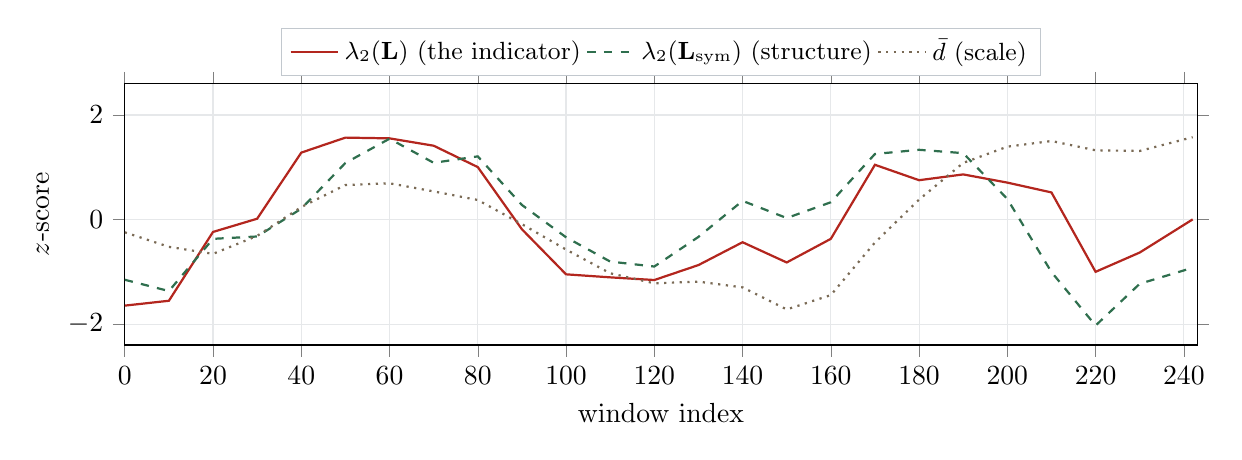
\begin{tikzpicture}
\begin{axis}[width=15.2cm,height=4.9cm,
  xlabel={window index}, ylabel={$z$-score},
  xmin=0,xmax=243,ymin=-2.4,ymax=2.6,
  grid=both,grid style={Rule!25},tick align=outside,
  legend columns=3,legend cell align=left,
  legend style={draw=Rule!60,font=\small,at={(0.5,1.03)},anchor=south}]
\addplot[BadRed,thick] coordinates {
(0,-1.647) (10,-1.554) (20,-0.237) (30,0.016) (40,1.281) (50,1.568) (60,1.554)
(70,1.413) (80,1.004) (90,-0.186) (100,-1.048) (110,-1.106) (120,-1.157)
(130,-0.871) (140,-0.434) (150,-0.821) (160,-0.369) (170,1.048) (180,0.753)
(190,0.864) (200,0.707) (210,0.519) (220,-1.000) (230,-0.631) (242,0.003)};
\addlegendentry{$\lambda_2(\Lap)$ (the indicator)}
\addplot[LapC,thick,dashed] coordinates {
(0,-1.152) (10,-1.368) (20,-0.369) (30,-0.324) (40,0.208) (50,1.083) (60,1.547)
(70,1.086) (80,1.209) (90,0.279) (100,-0.339) (110,-0.804) (120,-0.899)
(130,-0.332) (140,0.358) (150,0.029) (160,0.331) (170,1.255) (180,1.335)
(190,1.271) (200,0.394) (210,-1.005) (220,-2.028) (230,-1.229) (242,-0.922)};
\addlegendentry{$\lambda_2(\Lsym)$ (structure)}
\addplot[CorrC,thick,dotted] coordinates {
(0,-0.244) (10,-0.522) (20,-0.656) (30,-0.313) (40,0.239) (50,0.661) (60,0.694)
(70,0.539) (80,0.374) (90,-0.088) (100,-0.574) (110,-1.028) (120,-1.220)
(130,-1.188) (140,-1.298) (150,-1.720) (160,-1.446) (170,-0.439) (180,0.382)
(190,1.084) (200,1.395) (210,1.503) (220,1.325) (230,1.313) (242,1.576)};
\addlegendentry{$\bar d$ (scale)}
\end{axis}
\end{tikzpicture}
\caption{The indicator and its two ingredients, each standardised. The COVID
window is indices $150$--$173$. From index $\approx190$ (April 2020) the two
ingredients pull apart, structure relaxing sharply while scale keeps rising,
and the unnormalised $\lambda_2$, being a blend, stays elevated on scale alone.
That is the stretch in which Paper 1's strategy sits in cash through the recovery
and ends at $-0.011$ against buy-and-hold's $+0.078$.}
\end{figure}

\subsection*{Why this matters}

The degree sequence has to be combined with the structure somehow, and $\Lap$ and
$\Bmat$ use \textbf{different combination rules}:

\begin{center}\small
\renewcommand{\arraystretch}{1.25}
\begin{tabular}{@{}>{\raggedright\arraybackslash}p{4.2cm}
                  >{\raggedright\arraybackslash}p{11.2cm}@{}}
\toprule
$\Lap = \Dmat - \Amat$ &
degrees enter \textbf{additively}, on the diagonal: ``total connection, offset by
structure''. \\
$\Bmat = \Amat - \dvec\dvec^{\!\top}\!/2m$ &
degrees enter as a \textbf{rank-one null model}: ``does the observed structure
exceed what these degrees alone would predict, if edges were rewired at random?''
\\
\bottomrule
\end{tabular}
\end{center}

That second question is genuinely different, and by \S2 it is the \emph{only} thing
$\Bmat$ offers that $\Lap$ does not. It also explains, rather than merely
observing, why $\mu_N(\Bmat)$ keeps scoring well: it sits at the end of the
unnormalised modularity spectrum where the degree-dependent departure from the
normalised limit is largest.

% =====================================================================
\section{Final remarks and where to go next}
% =====================================================================

\subsection*{What was established}

The question as posed (find a modularity quantity carrying the same information
as the Fiedler value) has a negative answer, and the negative answer is the
deliverable. It \emph{closes} the direction rather than leaving it to be
re-attempted:

\begin{center}\small
\renewcommand{\arraystretch}{1.2}
\begin{tabular}{@{}lll@{}}
\toprule
\textbf{Route} & \textbf{Status} & \textbf{Why} \\
\midrule
normalised $\Bmat$ & \textcolor{BadRed}{closed by proof} &
$\Bn = \mathbf{I}-\Lsym-\mathbf{u}\mathbf{u}^{\!\top}$; same spectrum, same eigenvectors \\
$\mu_1$ with $\bar d$ substituted & \textcolor{BadRed}{closed as unsound} &
needs $\Dmat=d\mathbf{I}$; error is $89\%$ of the signal's sd \\
plain $\Bmat$, $\mu_1$ family & \textcolor{BadRed}{largely redundant} &
$|r|\ge0.79$ with $\mu_1$ for six of the leading candidates \\
plain $\Bmat$, negative end & \textcolor{LapC}{open} &
$\mu_N$ at $-0.668$ with $\mu_1$; no identity ties it to $\lambda_2$ \\
\bottomrule
\end{tabular}
\end{center}

\subsection*{The one surviving lead}

$\mu_N(\Bmat)$, the most negative modularity eigenvalue (the ``anti-community''
mode, sets of stocks actively avoiding one another), is the only candidate that is
neither tautological nor part of the $\mu_1$ family. Its case:

\begin{center}\small
\renewcommand{\arraystretch}{1.15}
\begin{tabular}{@{}lr@{}}
\toprule
$z$-scored COVID AUC & $0.775$ \quad(vs $\lambda_2$'s $0.759$) \\
redundancy with $\lambda_2$ ($z$-scores) & $+0.511$ \quad(against $-0.915$ for $\mu_1(\Bn)$) \\
redundancy with $\mu_1(\Bmat)$ (levels) & $-0.668$ \\
\textbf{independent test}, \texttt{reports/probe/} & best modularity signal at
\textbf{AUC $0.760$} vs $\lambda_2$'s $0.617$ \\
\quad\small(6{,}315 days, 360 stocks, 17 pre-registered crises) & \small$Q(t)$, Paper 3's
own indicator, scores $0.538$ \\
\bottomrule
\end{tabular}
\end{center}

The same quantity winning on two unrelated constructions is suggestive, and \S7
now supplies a mechanism rather than a coincidence. \textbf{But it is a lead, not a
result.} On FAAMUNG the difference is not significant ($\Delta$AUC $+0.015$ with
CI $[-0.115,\,+0.148]$), and $\mu_N$ fails the same sliding-event null that
$\lambda_2$ fails, at $p=0.345$. This dataset supports the framing; it cannot
support the claim.

\subsection*{Three possible directions}

The three headings below follow from the results above. Everything after each
heading is a suggestion rather than a recommendation, and the choice of which (if
any) to pursue is yours.

\begin{enumerate}[label=\textbf{D\arabic*.}]
\item \textbf{Validate $\lambda_2$ itself before comparing anything to it.} \S6
shows the incumbent indicator is not established on the data it was published on.

\emph{Suggestion.} One way to settle this would be a testbed with many events
scored under a single pre-registered detector, with a multiplicity correction. The
apparatus for that already exists in \texttt{reports/probe/} (17 crises over 25
years, where $\lambda_2$ scores $0.617$), so the cost would be small. It might be
worth doing before the others, since it would establish whether the rest of the
programme has a well-defined target at all, but that ordering is a judgement call.

\item \textbf{Characterise the departure from the normalised limit.} \S2 gives an
exact statement of what $\Bmat$ and $\Lap$ share, and \S7 shows the remaining
difference is carried entirely by the degree sequence, which is also where the
detection improvement appears.

\emph{Suggestion.} A natural object of study might therefore be the deviation
itself: how far adding degrees moves $\Bmat$ away from $\Bn$, in which modes, and
whether that displacement is the informative part. This looks to me like the
version of the original question that does not collapse into an identity, and so
perhaps the most promising candidate for a theory framework, though whether it is
worth formalising is better judged by you.

\item \textbf{Test $\mu_N(\Bmat)$ properly, gated on D1.}

\emph{Suggestion.} This would probably only be worth attempting on a testbed with
enough events to separate $0.775$ from $0.759$, which FAAMUNG is not. If it is
attempted, I would suggest pre-registering both the direction and the detector
before looking at the results, given how easily \S6 shows this data produces
apparent wins.
\end{enumerate}

\vspace{3mm}
\hrule
\vspace{2mm}
{\footnotesize
\textbf{Reproducing this.} \texttt{modularity\_indicator/} contains
\texttt{build\_series.py} (re-runs Algorithm 2, computes the menu),
\texttt{evaluate.py}, \texttt{robustness.py}, \texttt{significance.py},
\texttt{figures.py}, and \texttt{report\_numbers.py}, which prints every number in
this report. Run in order with \texttt{../.venv/bin/python}; total runtime under a
minute. Nothing in \texttt{paper1\_gmrf\_laplacian/} is modified; it is read only.
Companion documents: \texttt{reports/progress\_report.tex} (running log) and
\texttt{reports/2026-08-19\_discrepancy\_explained.tex} (the earlier
three-paper exploration).
\par}

\end{document}
